% Use class option [extendedabs] to prepare the 1-page extended abstract.
\documentclass[extendedabs]{bmvc2k}
\usepackage[colorlinks = true,
            linkcolor = blue,
            urlcolor  = blue,
            citecolor = blue,
            anchorcolor = blue]{hyperref}
\usepackage{kotex}
% for the fancy \koTeX logo
\usepackage{kotex-logo}
\usepackage{mathtools}  % brings in amsmath, also some improvements
\usepackage{amssymb} % brings in amsfonts, incl \square
% Document starts here
\begin{document}


\title{semantic segmentation pre-report}
\addauthor{
Taehun Kim$^{1}$
}{}{1}

\addinstitution{
$^1$ Department of Computer Science and Engineering, Pusan National University.  
}
 

\maketitle
\noindent

\section{Introduction}
This report summarizes two well-known semantic segmentation papers, Fully Convolutional Network(FCN)\cite{fullyconvnet} and Learning Deconvolution Network\cite{learndeconv}.

\section{Fully Convolutional Network}
Typical convolutional network for image classification has fully connected layers,which take fixed-size inputs and throw away spatial information. However, By replacing fully connected layers with convolutional layers like \ref{FCN}, We can make fully convolutional network that takes input of arbitary size and produce fixed-channel outputs.

\begin{figure}[t]
	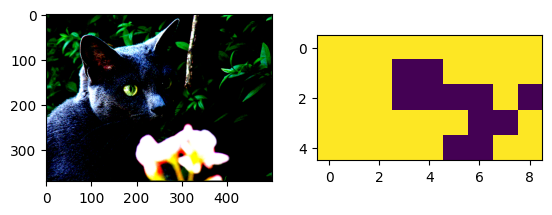
\includegraphics[width=\linewidth]{images/fig2.png}
	\caption{
		changing fully connected layers to convolution layers enables remaining the spatial information}
	\vspace{-2mm}
 \label{FCN}
\end{figure}

\subsection{Upsampling is backwards strided convolution}
After the input image passes through the convolution layer, its width and height decrease. As a result, the output feature map becomes coarser compared to the original image. Since segmentation needs to be performed at the pixel level of the original image, It is necessary to convert the feature map to a dense map with a size similar to the original image.

A way to upsample is $backwards convolution$(or $deconvolution$). this simply reverses the forward and backward passes of convolution. In other words, forward pass calculate $n\times n$ values from one value using filter. this method can upsample feature map to original image size, which enables getting pixelwise loss.

\subsection{Architecture}
The paper replaces classifiers into FCNs(i.e., a $1\times1)$ convolutional layer for each classes including background, and upsampling layer), and augment feature maps with in-network upsampling and pixelwise loss. Then, they train model by fine-tuning. Finally, they build a skip architecture that combines coarse information to refine prediction.

\subsection{Combining what and where}
In VGG16\cite{vgg}, the final feature map is 32 times smaller than the input image. This limits the scale of detail in the upsampled output.

The paper address this by combine the final prediction layer with lower layers. In paper, there are 3 upsampled prediction(FCN-32s, FCN-16s, FCN-8s). FCN-32s is prediction that upsample $1\times1$ map by a factor of 32. FCN-16s is prediction that upsample $2\times2$ by a factor of 16. FCN-8s is prediction that upsample $4\times4$ by a factor of 8. In other words, FCN is applied after 3,4 and 5 maxpooling of VGG-16\cite{vgg}. Combining fine layer(FCN-8s) and coarse layers(FCN-32s) lets the model make local prediction with respect global structure. this called \textit{Deep jet}. In figure \ref{skip}, FCN-8s has most detailed information.

\section{Learning Deconvolution Network}
Learning Deconvolution Network paper\cite{learndeconv} says semantic segmentation based on FCN\cite{fullyconvnet} has limitations. First, pixels that belong to the large object may have inconsistent labels if the large object contains small object. Also, small objects are often classified as background. This is due to the fixed-size receptive field.

To overcome such limitations, The paper\cite{learndeconv} has different strategy. First, they learn a multi-layer deconvolution network. this network consists of deconvolution, unpooling and ReLU layers. Second, the trained network is applied to object proposals. this method is free from scale issues.

\subsection{Architecture}
Figure \ref{learndeconv} is entire architecture of learning deconvolution network. this network has two parts, one is convolution and another is deconvolution network. the convolution part extract features, and deconvolution network produce segmentation from extracted features.

The final output of this network has same size(width and height) to input image, and has same channel to the number of classes, indicating probability of each pixel's classes.

The paper uses VGG-16\cite{vgg}(without last classification layers) for convolution part. convolution network has 13 conv layers, and 2 fully connected layers are at the end for class projection. The deconvolution network is a mirrored version of the convolution network. The convolution layer is replaced to deconvolution layer(\ref{deconvolution}), and the maxpooling layer is replaced to unpooling layer(\ref{unpooling}) in deconvolution network.
\subsection{Deconvolution Network}
Deconvolution network generates object segmentation mask from coarse feature map.
\subsubsection{Unpooling} \label{unpooling}
The unpooling layers perform the reverse operation of pooling. To implement the unpooling, The paper\cite{learndeconv} records the location of selected value during maxpooling, and place each activation back to its original location during unpooling. This layer generate enlarged, but sparse map.
\subsubsection{Deconvolution} \label{deconvolution}
The deconvolutional layer associate a single input activation with multiple outputs. In other words, forward pass calculate $n\times n$ values from one value using $n\times n$ filter. lower layers capture overall shape of an object, and higher layers encoded fine details. Coarse-to-fine object structures are reconstructed through the deconvolution layers.
\subsection{System Overview}
This network takes a sub-image(proposals) potentially containing objects as input. Then the network aggregate outputs of all proposals to the original image space. It reduces search space and enables identifying fine-details and handling objects in various scales.
\subsection{Training}
This network uses the batch normalization to reduce the internal-covariate-shift. Also, It train on two-stage. First, they use images that object is centered through crop the image. Second, they use more challenge examples like proposals that overlapped with ground-truth segmentations(i.e., the object is cropped or in edge)
\begin{figure}[t]
	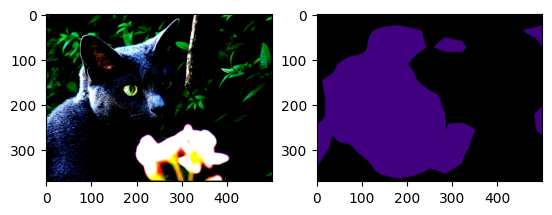
\includegraphics[width=\linewidth]{images/fig3.png}
	\caption{
		Refining fully convolutional nets by fusing information from layers with different strides}
	\vspace{-2mm}
 \label{skip}
\end{figure}
\begin{figure}[t]
	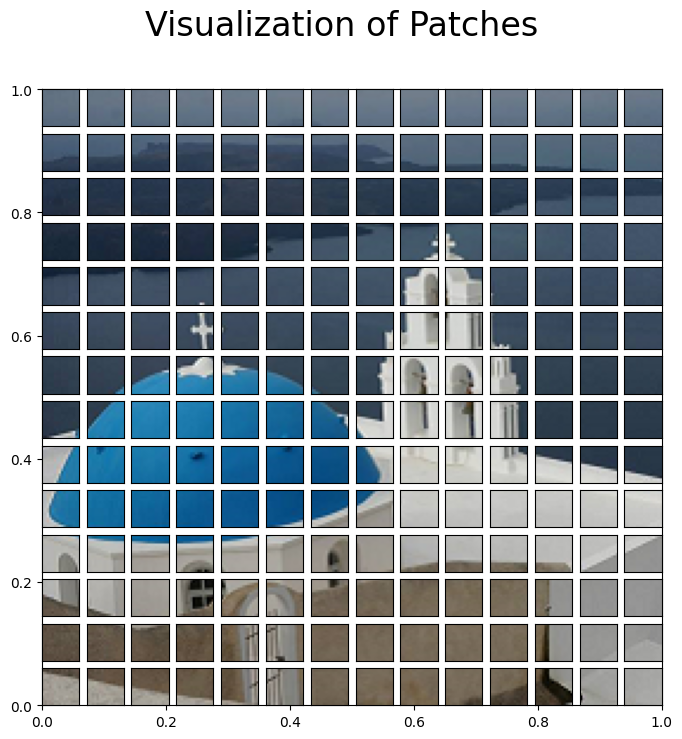
\includegraphics[width=\linewidth]{images/fig4.png}
	\caption{
		Overall architecure of the learning deconvolution network.}
	\vspace{-2mm}
 \label{learndeconv}
\end{figure}
\begin{figure}[t]
	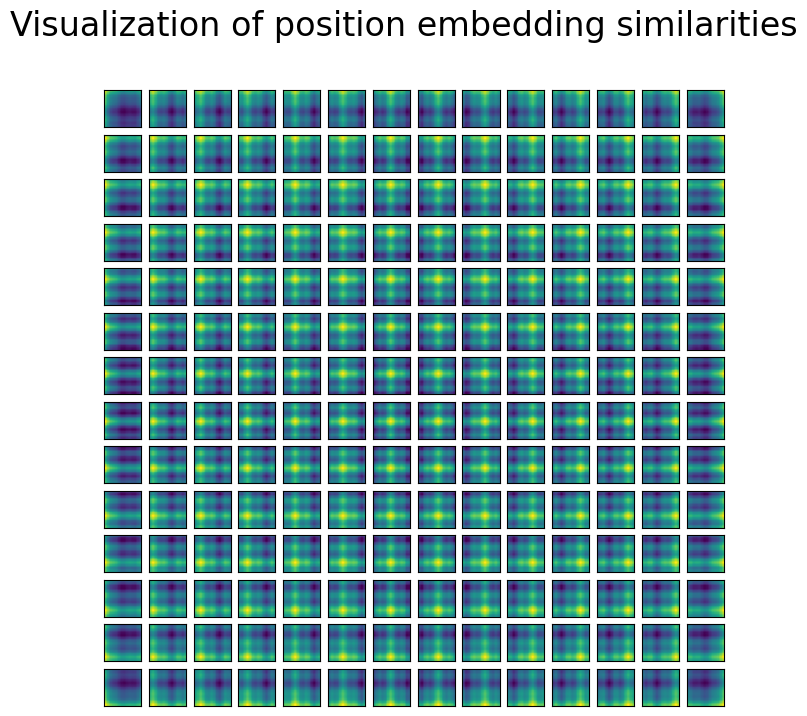
\includegraphics[width=\linewidth]{images/fig5.png}
	\caption{
		Comparison between FCN(middle) and learning deconvolution network(right). learning deconvolution network detects more precisely.}
	\vspace{-2mm}
 \label{compare_FCN_Deconv}

\end{figure}
\section{Conclusion}
We summarize two well-known semantic segmentation papers, Fully Convolutional Network(FCN)\cite{fullyconvnet} and Learning Deconvolution Network\cite{learndeconv}.

Fully convolutional Network(FCN)\cite{fullyconvnet} uses Uppooling, fully convolutional network, skip connection(Deep jet). Learning Deconvolution Network uses deconvolution network that consists of unpooling layers and deconvolution layers. These method enables pixel-wise semantic segmentation.
\newpage
\bibliography{egbib}

\end{document}
